\documentclass[autodetect-engine,dvi=dvipdfmx,ja=standard,
               a4j,11pt]{bxjsarticle}

\RequirePackage{geometry}
\geometry{reset,paperwidth=210truemm,paperheight=297truemm}
\geometry{hmargin=.75truein,top=20truemm,bottom=25truemm,footskip=10truemm,headheight=0mm}
%\geometry{showframe} % 本文の"枠"を確認したければ，コメントアウト
\usepackage{graphicx}
\usepackage{fancyvrb}
\usepackage{spverbatim}
\usepackage{amsmath}

\renewcommand{\theFancyVerbLine}{\texttt{\footnotesize{\arabic{FancyVerbLine}:}}}

\title{画像処理実験 第3回}
\author{学生番号: 09B24490\\
        加藤弘都 (KATO, HIROTO)}
\date{\number\year 年\number\month 月\number\day 日}

%%======== 本文 ====================================================%%
\begin{document}
\maketitle
% 目次つきの表紙ページにする場合はコメントを外す
%{\footnotesize \tableofcontents \newpage}

%--------------------------------------------------------------------%
\section{課題3} \label{sec:abstract}

\subsection{[3-1]　\texttt{A}，\texttt{b}を考える} \label{3-1}

\verb|A|，\verb|b|は定義より，\verb|main|関数で定義した行列\verb|w|を用いて以下のように表せる．


\begin{Verbatim}[numbers=left, xleftmargin=10mm, numbersep=6pt,
                    fontsize=\small, baselinestretch=0.8]
  A[i*2+0,0]=w[i, 0]
  A[i*2+0,1]=w[i, 1] 
  A[i*2+0,2]=1
  A[i*2+1,2]=0
  A[i*2+0,3]=0
  A[i*2+1,3]=w[i, 0] 
  A[i*2+0,4]=0
  A[i*2+1,4]=w[i, 1]
  A[i*2+0,5]=0
  A[i*2+1,5]=1
  A[i*2+0,6]=-1 * w[i,0] * w[i, 2]
  A[i*2+1,6]=-1 * w[i,0] * w[i, 3]
  A[i*2+0,7]=-1 * w[i,1] * w[i, 2]
  A[i*2+1,7]=-1 * w[i,1] * w[i, 3]

  b[i*2+0  ]=w[i,2]
  b[i*2+1  ]=w[i,3]
\end{Verbatim}


\subsection{[3-2]}

\subsubsection{[3-1]で求めた\texttt{H}を用いた画像合成}

[2-2]で作成したコードを参考に作成する．以下のように\ref{3-1}で作成した関数\verb|calcHomography(w)|
で求めた変換行列を行列\verb|m10|に格納すると画像は\ref{3-1-1}のようになった．
４つの点は密集していて，４つの点がある中心付近は正確であるが，離れるほどぼやけていることがわかる．

\begin{Verbatim}[numbers=left, xleftmargin=10mm, numbersep=6pt,
                    fontsize=\small, baselinestretch=0.8]
  w=np.array(
     [[256, 218, 371, 230],
      [347, 220, 463, 230],
      [263, 367, 383, 379],
      [413, 315, 530, 327]])
  m10=calcHomography(w)
\end{Verbatim}

\begin{figure}[h]
 \centering
 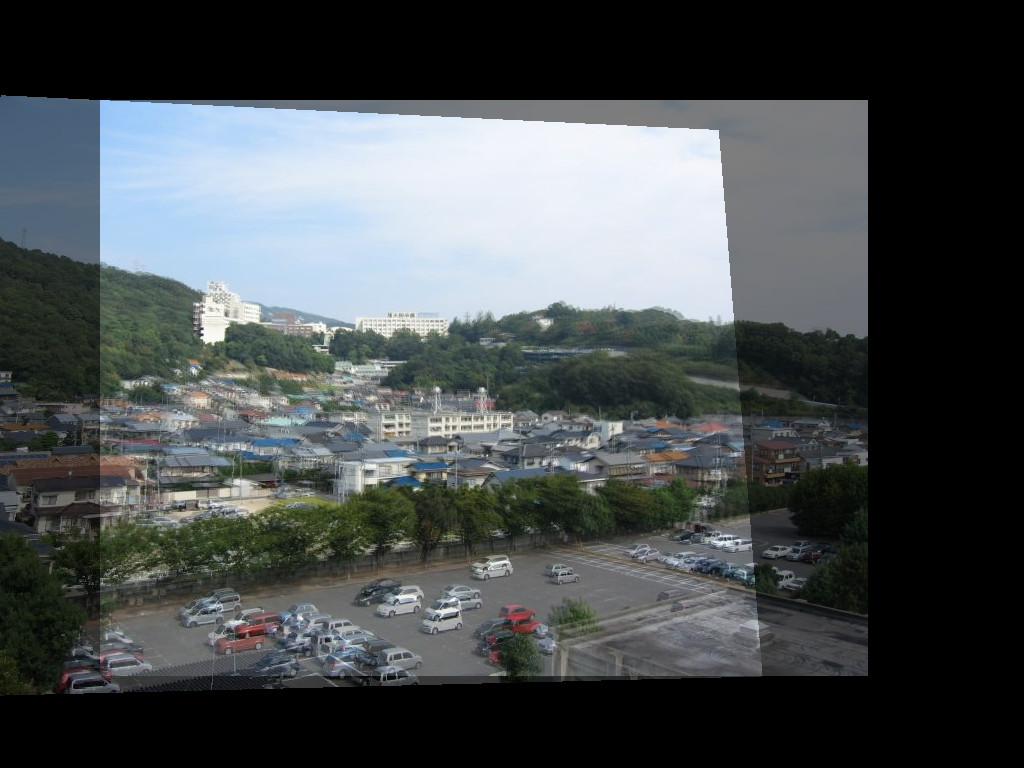
\includegraphics[scale=.15]{../3class/3-1-1.jpg}
 \caption{求めたHで生成した画像}
 \label{3-1-1}
\end{figure}

\subsubsection{合成画像の品質向上}

近い4点の座標を選択するとその箇所は比較的に正確に合成できるが，
離れた箇所ほどずれてしまう．
このことから，遠く離れた4点の座標を選択して品質向上を図る．
以下のコードは新しく選んだ４つの点を\verb|w|に格納している．
生成した画像は\ref{3-1-2}の左側である．
生成した画像\ref{3-1-2}は画像\ref{3-1-1}よりも画質が悪いように感じる座標を
うまく対応できなかったのではないかと考える．

また，これらの８つの座標の\verb|w|をもちいて画像を作成すると図\ref{3-1-2}の右側のようになる．
図\ref{3-1-2}の左側の画像は中心付近はぼやけているが，離れるほど正確に表現できていることがわかる．
図\ref{3-1-2}の右側の画像ではこれまでの画像に比べて全体的に正確な画像になった．

\begin{Verbatim}[numbers=left, xleftmargin=10mm, numbersep=6pt,
                    fontsize=\small, baselinestretch=0.8]
  w=np.array(
     [[113,188,231,201],
      [281,513,398,521],
      [621,218,742,223],
      [573,437,697,448]])
\end{Verbatim}

\begin{figure}[h]
 \centering
 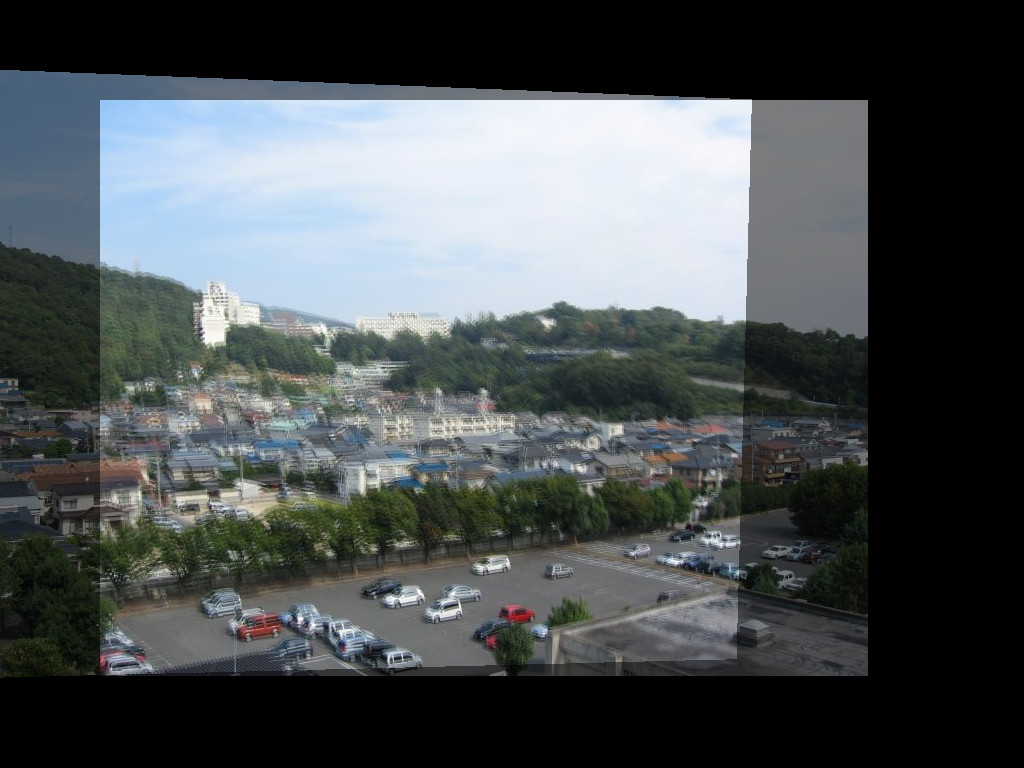
\includegraphics[scale=.15]{../3class/3-1-2.jpg}
 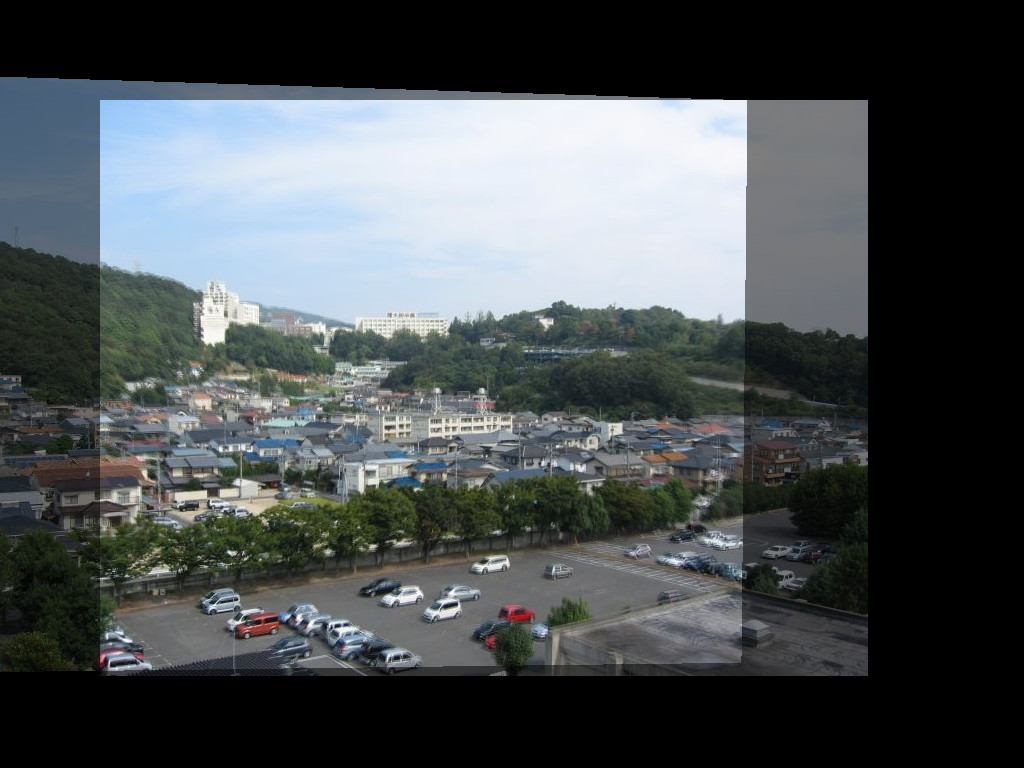
\includegraphics[scale=.15]{../3class/3-1-3.jpg}
 \caption{求めたHで生成した画像}
 \label{3-1-2}
\end{figure}

\subsubsection{自分で撮影した画像}

同一の視点から方向を変えて撮影した二枚の画像を準備する．
それらの画像から８つの座標を選択し，合成画像を生成すると図\ref{3-1-2}のようになる．
合成画像を見ると，様々な８つの点を選択したため，全体的に正確な画像を作成できたと考える，
具体的にはパソコンに表示されている文字も重なっている部分が多く，文章が読めるほどである．

\begin{figure}[h]
 \centering
 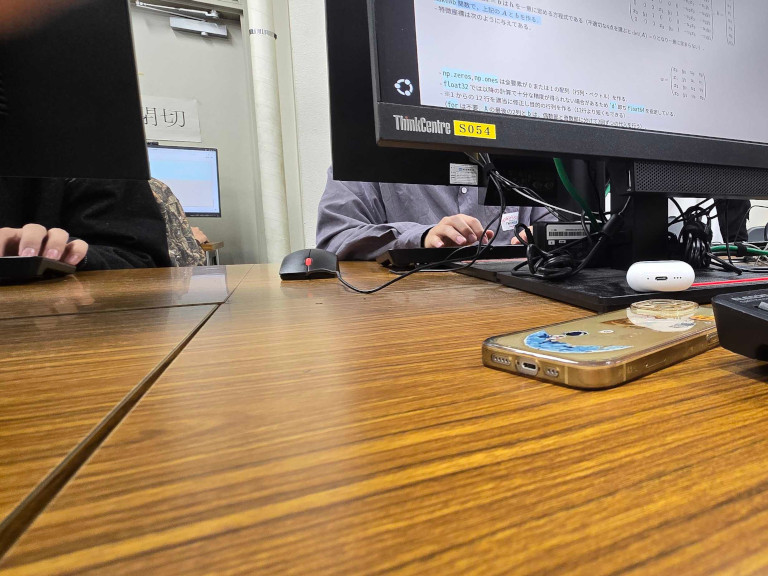
\includegraphics[scale=.5]{../3class/my1.jpg}
 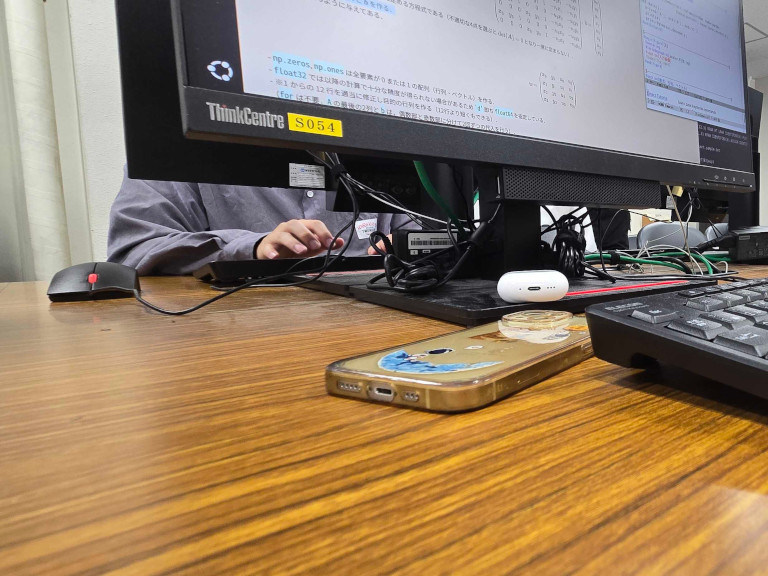
\includegraphics[scale=.5]{../3class/my2.jpg}
 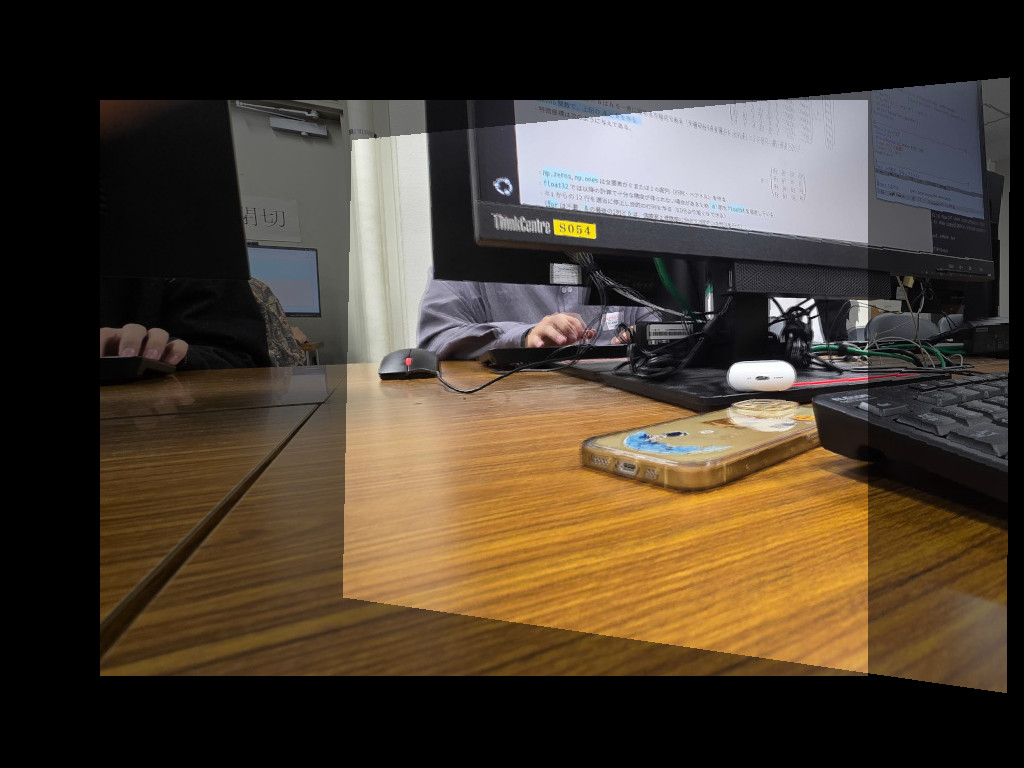
\includegraphics[scale=.15]{../3class/3-2-4.jpg}
 \caption{自分で撮影した画像（左，中央）と合成画像}
 \label{3-1-2}
\end{figure}



% \subsubsection{第 1 回の「適当な処理 7」と\texttt{afn}の比較，\texttt{afn2}, \texttt{afn3}}

% まず，第 1 回の「適当な処理 7」と比較する．
% 比較したとき，\verb|[2.1 geom]|は回転角度，拡大倍率，\verb|c|，\verb|s|を\verb|main|関数で定義していて，
% \verb|afn|関数では\verb|u|，\verb|v|と新しい画像を定義している．
% 両者の処理に違いはなく，定義されている関数が異なるだけだと考える．
% そのため，両者とも射影変換を用いて45度回転させて，3.5倍に拡大している．

% 次に\verb|afn2|関数について説明する．
% この関数では，\verb|afn|関数と同じ処理をしている．
% \verb|afn|関数では\verb|main|関数内の定義より画像の\verb|(550,220)|座標を
% 基準に\verb|[-150:150,-150:150]|の範囲の画像を指定していた．
% しかし，\verb|afn2|関数では，\verb|main|関数内で\verb|a|に指定した行列をかけて，
% \verb|a|で指定していた\verb|(550,220)|座標から\verb|(-550, -220)|の平行移動をさせて，
% \verb|(0,0)|を基準に画像を指定しようとしている．
% これにより\verb|afn2|関数内で\verb|[70:370,400:700]|のように
% 画像の範囲を直接指定して拡大・回転させている．

% 最後に\verb|afn3|関数では黒の背景部分を出力せず，
% 画像のみ画面に出力するようにしている．
% \verb|u|，\verb|v|が画像の中にあるときに\verb|True|，
% そうでないときに\verb|False|を格納する配列\verb|m|を定義し，
% \verb|m==True|のときのみ\verb|im|に格納している．\verb||\verb||

% \subsubsection{射影変換の関数の実装}

% \verb|afn3|関数をもとに以下のような射影変換の関数\verb|proj|を実装した．
% \verb|afn3|では\verb|z|を考えていなかったため\verb|z_|を求め，
% \verb|u=x_/z_|，\verb|v=y_/z_|に変更する．

% \begin{Verbatim}[numbers=left, xleftmargin=10mm, numbersep=6pt,
%                     fontsize=\small, baselinestretch=0.8]
% def proj(dw,dh, src, a):



%  im=np.zeros((dh,dw,3),'f')

%  y ,x =np.mgrid[0:dh,0:dw]                   # (i)

%  # z_を追加-----
%  x_,y_,z_= a[0,0]*x+a[0,1]*y+a[0,2], \
%         a[1,0]*x+a[1,1]*y+a[1,2], \
%         a[2,0]*x+a[2,1]*y+a[2,2]

%  # z_を追加-----
%  u,v=x_ / z_, \
%     y_ / z_

%  m = (0<=u)&(u<src.shape[1])&(0<=v)&(v<src.shape[0]) # (iv)
%  # 画像内の座標しか参照しないため，画像を拡大できる

%  im[y[m],x[m]]= src[v[m].astype('i'),
% 		    u[m].astype('i')]        # (iii) int型でやっている

%  return im
% \end{Verbatim}


% \subsubsection{変換行列の変化による画像の相違}

% 変換行列を変更したとき，図\ref{2-1-1}のようになる．左側は変更前で，右側は変更後である．

% \verb||\verb||\verb||\verb||\verb||\verb||\verb||\verb||

% \begin{figure}[h]
%  \centering
%  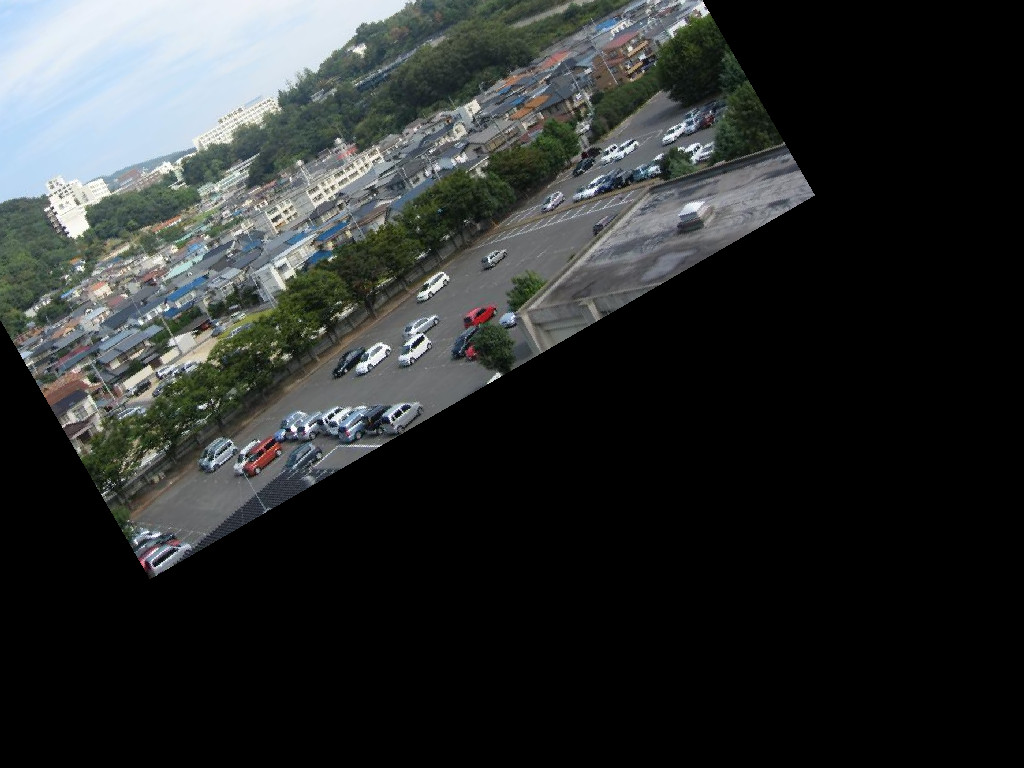
\includegraphics[scale=.15]{2class/2-1-1.jpg}
%  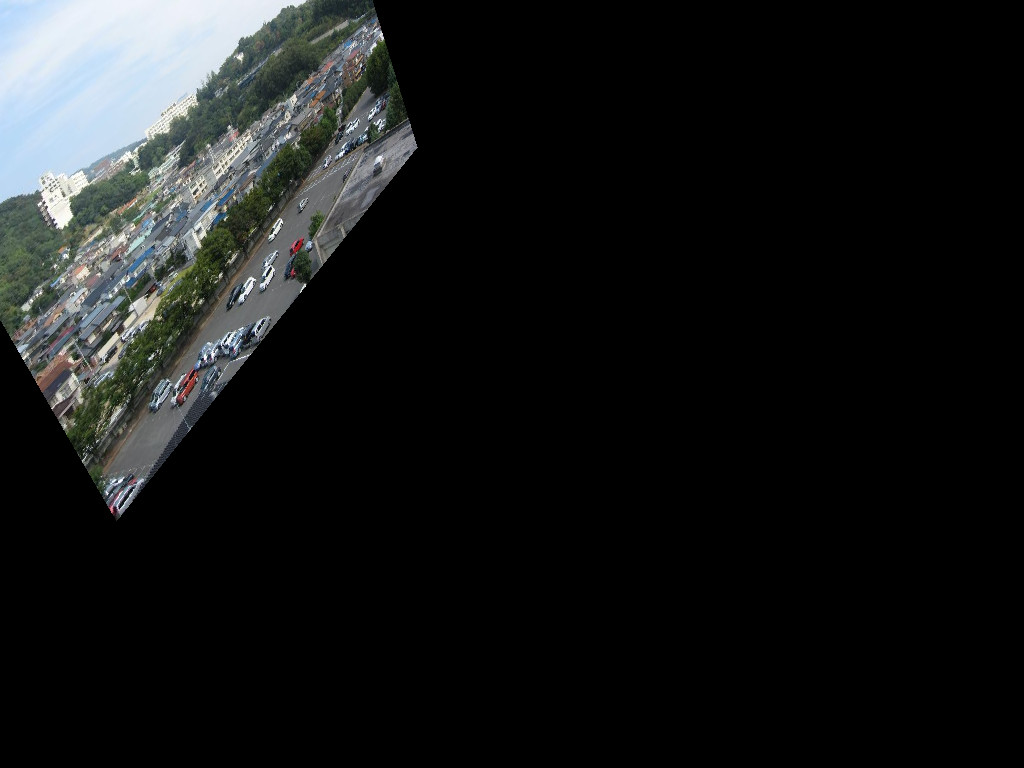
\includegraphics[scale=.15]{2class/2-1-2.jpg}
%  \caption{変換行列の変化による２つの画像（左は変更前で右は変更後）}
%  \label{2-1-1}
% \end{figure}

% ２つの画像を比較すると，
% 変更前の画像の方が見える画像の面積が広く，画像が見える角度が変化していることがわかる．

% \subsubsection{回転・拡大/縮小行列A の一般形}

% m倍に拡大し，t度回転させるとき，「原画像の座標(u,v)を出力画像の座標(x,y)に変換する
% 回転・拡大/縮小行列」A の一般形は以下のようになる．

% \[
% A = 
% \begin{pmatrix}
% \frac{\cos t}{m} & - \frac{\sin t}{m} & 0 \\
% \frac{\sin t}{m} & \frac{\cos t}{m} & 0 \\
% 0 & 0 & 1 \\
% \end{pmatrix}
% \]

% まず点\verb|(p,q)|を中心とする\verb|m|倍の拡大縮小を行う．以下のように\verb|a|を定義するとき，
% \verb|t=0|，\verb|p=0|，\verb|q=0|という条件のときの\verb|m|が$1$と$0.5$の違いを図\ref{2-1-2}
% に示す．図のように\verb|m|の値に応じて画像が拡大・縮小していることがわかる．

% \begin{Verbatim}[numbers=left, xleftmargin=10mm, numbersep=6pt,
%                     fontsize=\small, baselinestretch=0.8]
%   a=np.array([[ c, -s, q],
%   	      [ s,  c, p],
%   	      [ 0,  0,   1]])
% \end{Verbatim}


% \begin{figure}[h]
%  \centering
%  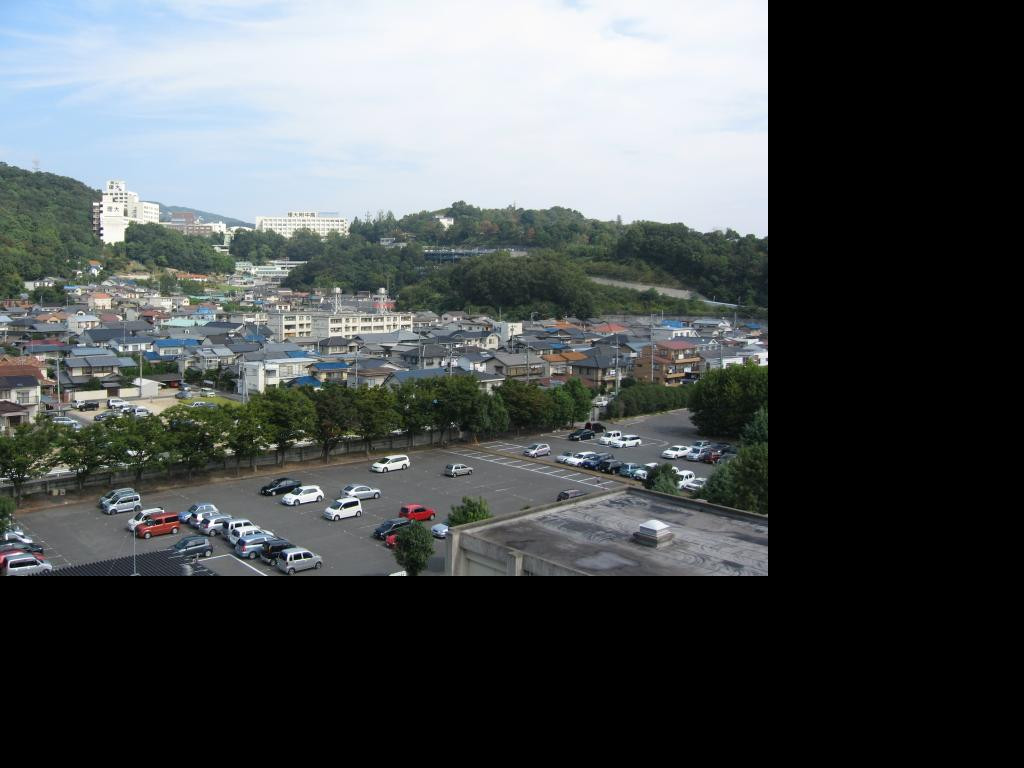
\includegraphics[scale=.15]{2class/2-1-3.jpg}
%  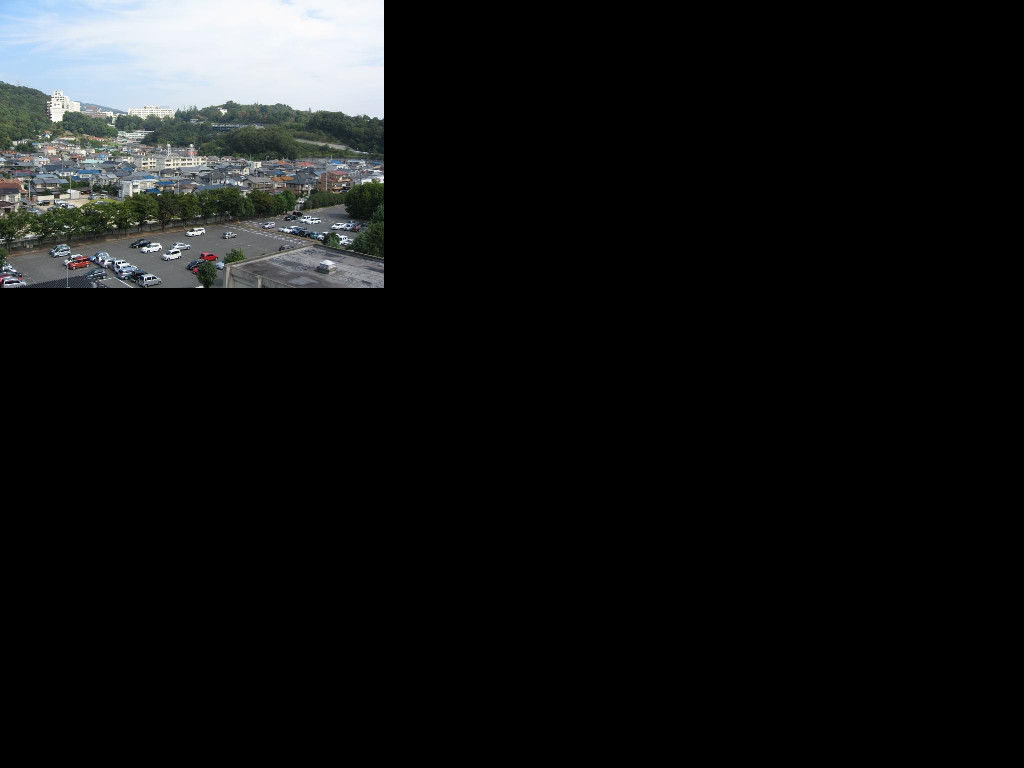
\includegraphics[scale=.15]{2class/2-1-4.jpg}
%  \caption{\texttt{m}が$1$（左）と$0.5$（右）のときの画像}
%  \label{2-1-2}
% \end{figure}

% 次に，点\verb|(p,q)| を中心とする角度\verb|t|の回転を行う．
% \verb|m=1|，\verb|p=0|，\verb|q=0|という条件のときの\verb|t|が$0$と$\frac{\pi}{4}$
% の違いを図\ref{2-1-3}に示す．
% 図のように\verb|t|の値によって画像が$\frac{\pi}{4}$だけ回転していることがわかる．

% \begin{figure}[h]
%  \centering
%  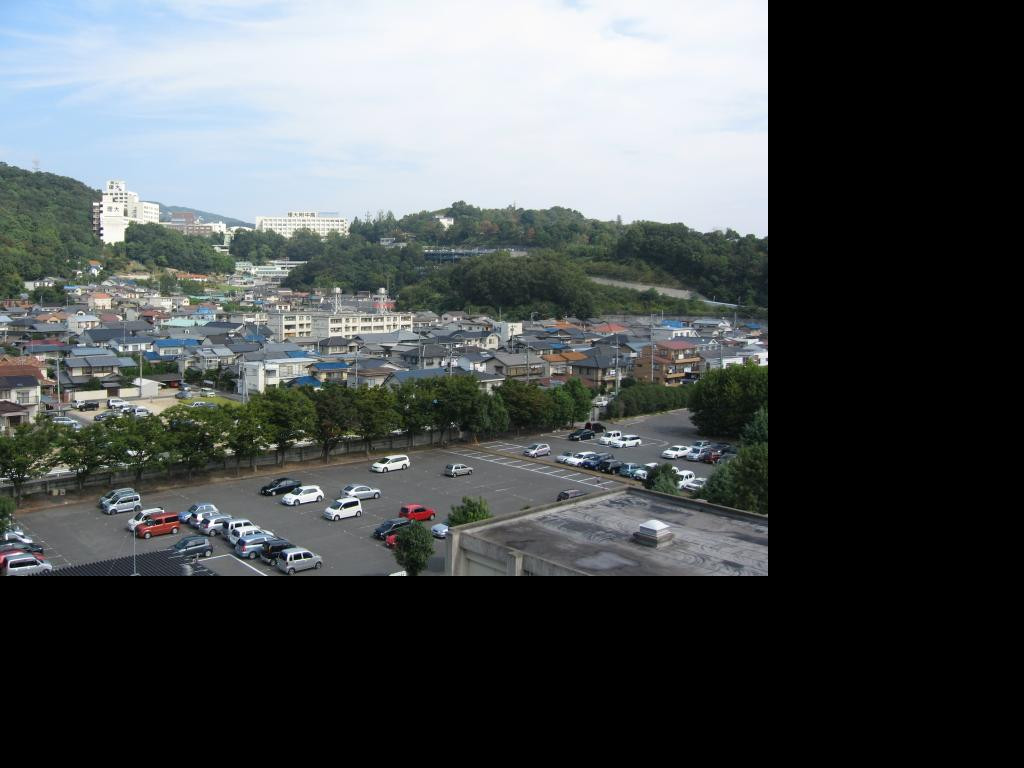
\includegraphics[scale=.15]{2class/2-1-3.jpg}
%  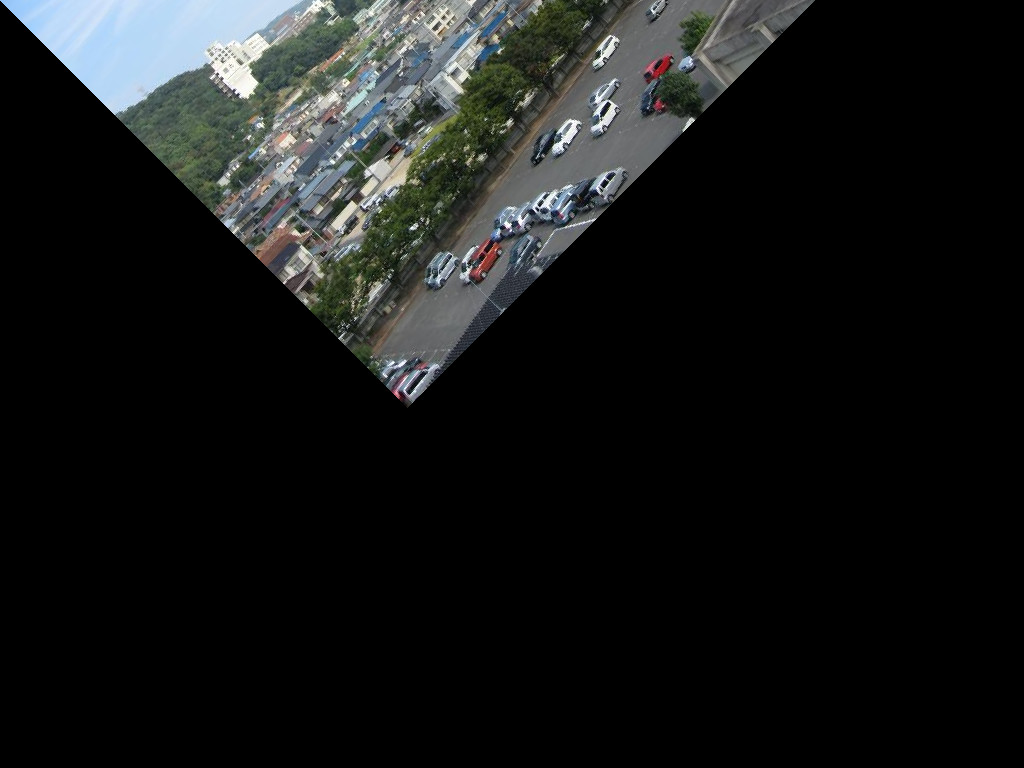
\includegraphics[scale=.15]{2class/2-1-5.jpg}
%  \caption{\texttt{t}が$0$（左）と$\frac{\pi}{4}$（右）のときの画像}
%  \label{2-1-3}
% \end{figure}


% \subsection{[2-2]}
% \subsubsection{\texttt{m0d}の変化による位置関係}

% \verb|m0d|関数を変更したとき，２つの画像の位置関係が変化しないことを確かめる．
% 図\ref{2-1-4}では以下のように変更をした．

% \begin{Verbatim}[numbers=left, xleftmargin=10mm, numbersep=6pt,
%                     fontsize=\small, baselinestretch=0.8]
%   # 左の画像（もとのm0d関数）
%   m0d=np.array([[ 1,0,-100 ],
%                 [ 0,1,-100 ],
%                 [ 0,0,1 ]],'f')
%   # 中央の画像（拡大させた）
%   m0d=np.array([[ .5,0,-100 ],
%                 [ 0,.5,-100 ],
%                 [ 0,0,1 ]],'f')
% 　# 右の画像（平行移動をなくした）
%   m0d=np.array([[ 1,0,0 ],
%                 [ 0,1,0 ],
%                 [ 0,0,1 ]],'f')
% \end{Verbatim}


% \begin{figure}[h]
%  \centering
%  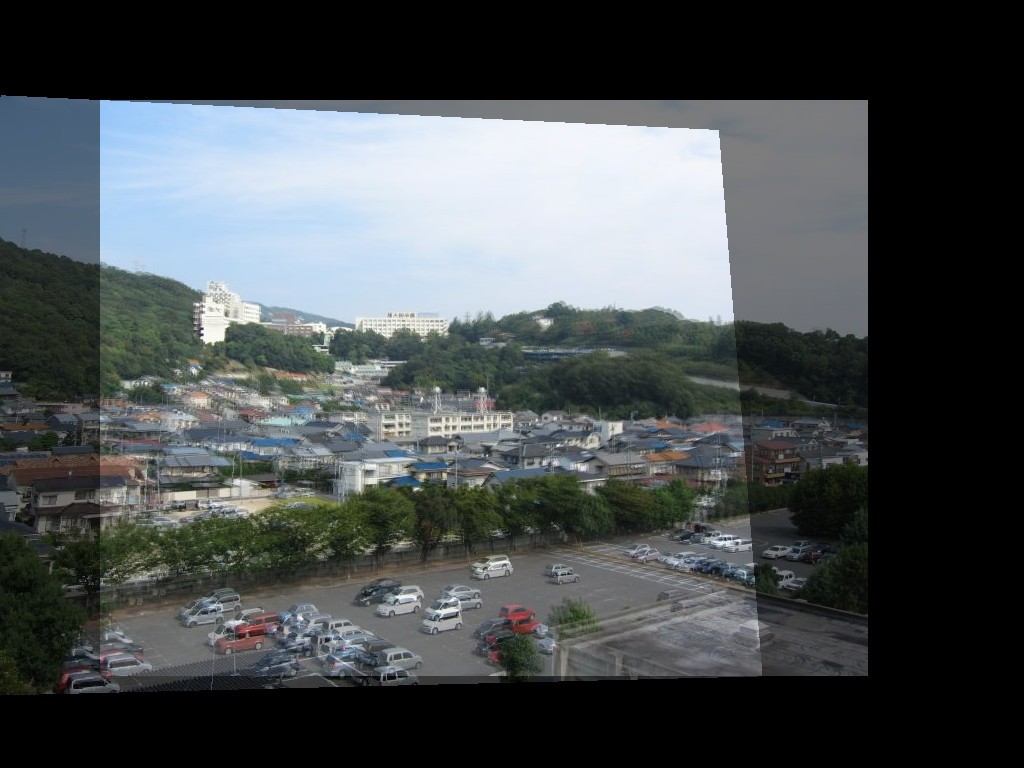
\includegraphics[scale=.1]{2class/2-1-6.jpg}
%  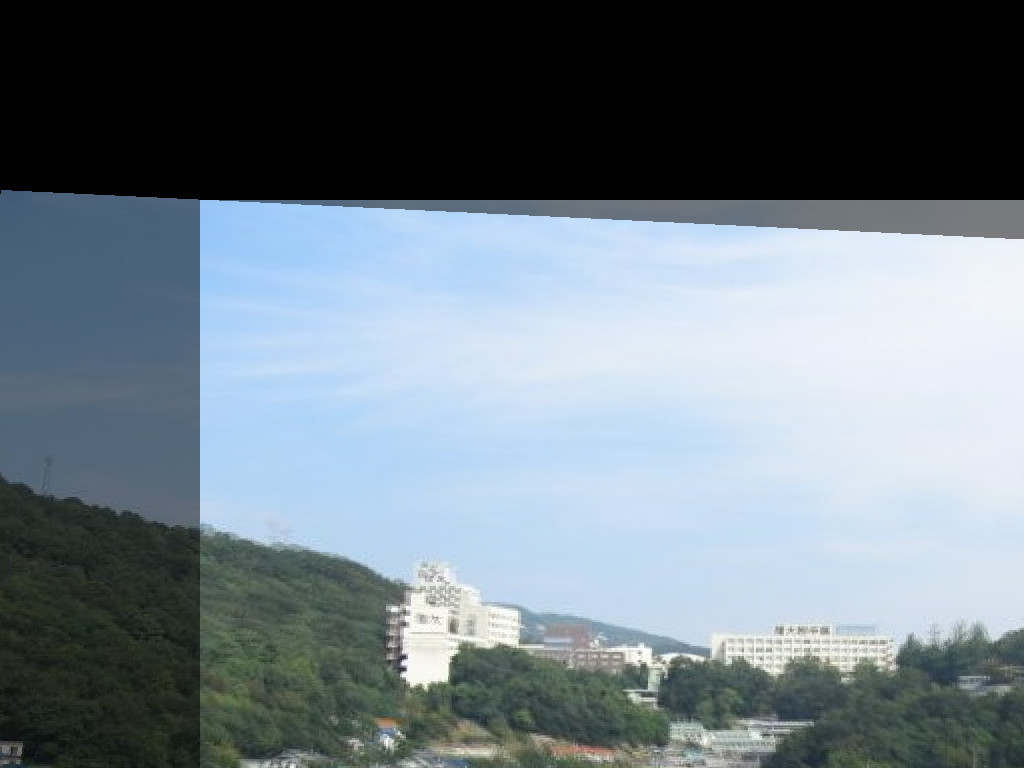
\includegraphics[scale=.1]{2class/2-1-7.jpg}
%  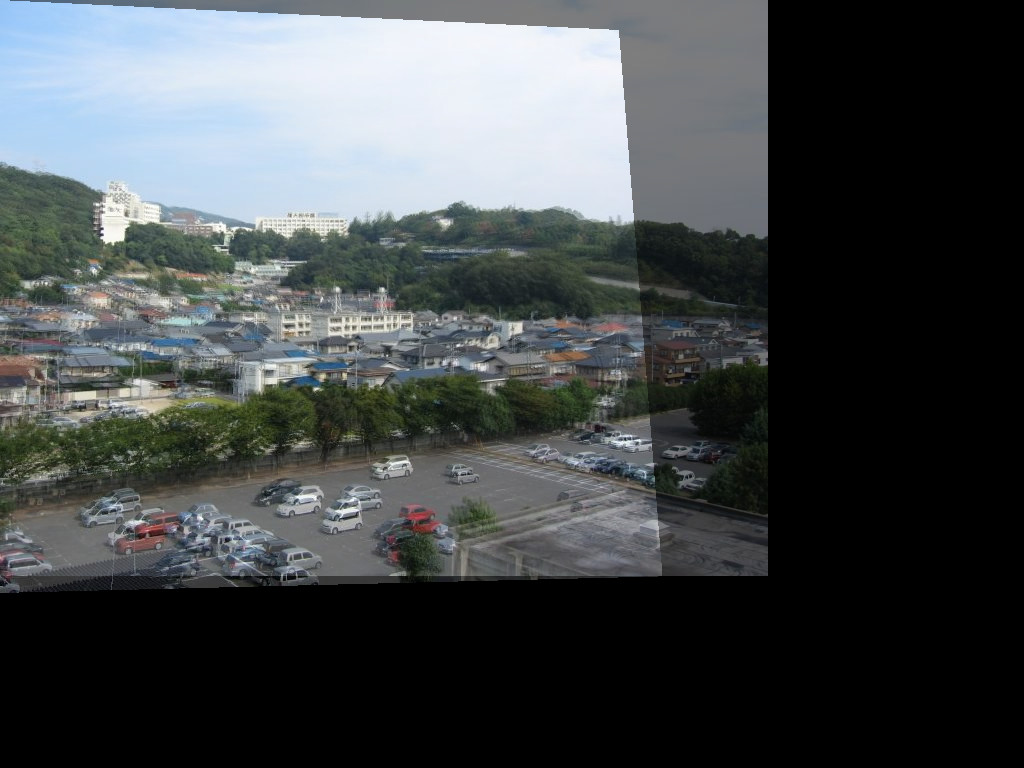
\includegraphics[scale=.1]{2class/2-1-8.jpg}
%  \caption{\texttt{m0d}関数を変更した３つの画像}
%  \label{2-1-4}
% \end{figure}

% これらの画像の変化を比較したとき，拡大，平行移動させても２つの画像の位置関係は
% 変化していないことがわかる．

% \subsubsection{ずれのない合成画像}
% 次に\verb|m10|関数を変更し，ずれのない合成画像を生成する．
% \verb|m10|関数を以下のように変更したとき，生成される画像は
% 図\ref{2-1-5}のようになる．

% \begin{Verbatim}[numbers=left, xleftmargin=10mm, numbersep=6pt,
%                     fontsize=\small, baselinestretch=0.8]
%   m10=np.array(['''
% 0.949961 0.007558 127.986108
% -0.046213 0.996315 27.732034
% -0.000113 -0.000012 1.040526 '''.split()]).astype('f').reshape(3,3)
% \end{Verbatim}

% \begin{figure}[h]
%  \centering
%  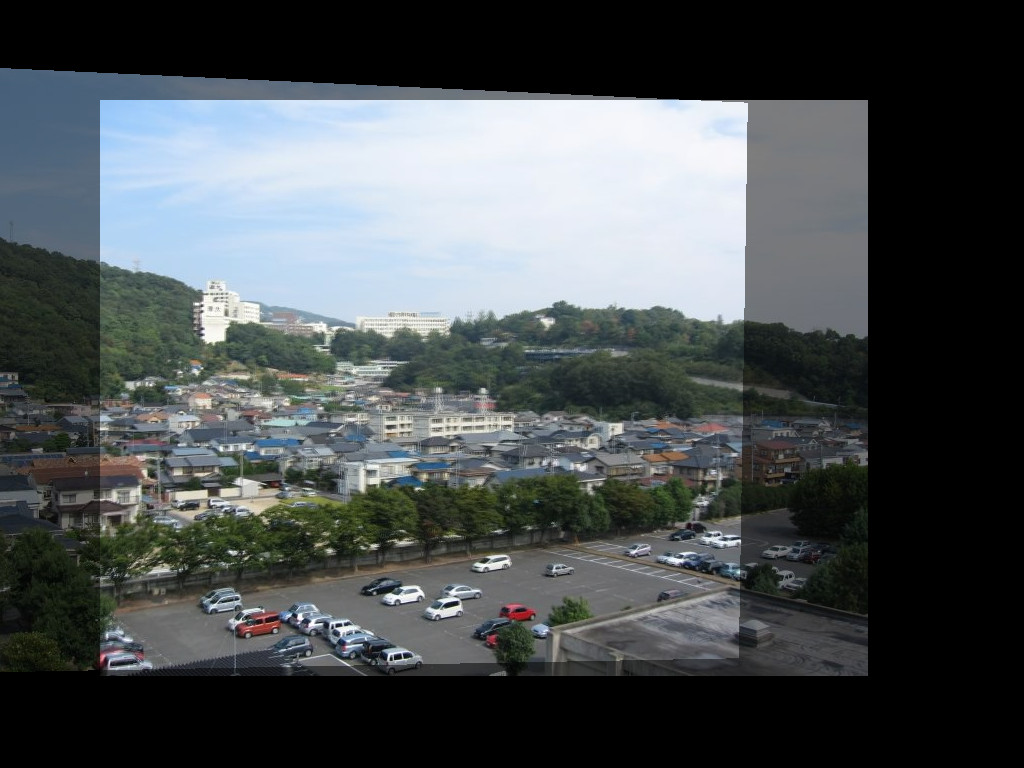
\includegraphics[scale=.15]{2class/2-1-9.jpg}
%  \caption{ずれのない合成画像}
%  \label{2-1-5}
% \end{figure}


%--------------------------------------------------------------------%


%--------------------------------------------------------------------%
% \section{数式: 行列，ベクトル}

% \newcommand\bA{\mbox{\boldmath$A$}}
% \newcommand\bb{\mbox{\boldmath$b$}}
% 太字$\bA$を使えるように定義した．
% $\bA^{-1}\bb$等，使う文字を newcommand で定義して使う．

% \boldsymbol{A} は使えない


%--------------------------------------------------------------------%
\section{感想}

画像合成を正確にやりまくれば360度カメラとかも作れそうだなーと感じた．

%--------------------------------------------------------------------%
% 参考文献
%   以下は，書き方の例である．実際に，参考にした書籍等を見て書くこと．
%   本文で引用する際は，\cite{book:algodata}などとすればよい．
\begin{thebibliography}{99}
  % \bibitem{book:algodata} 平田富雄，アルゴリズムとデータ構造，森北出版，1990.
  % \bibitem{book:label2} 著者名，書名，出版社，発行年.
  % \bibitem{www:label3} WWWページタイトル，\spverb!https://example.of.too.long.url.jp/you.must.use.spverb/and.insert. a.space.somewhere.to.avoid.overfull.html!，アクセス日.
\end{thebibliography}

%--------------------------------------------------------------------%
\end{document}
